We present a unified infrastructure to support Deep FAIR for relational mathematical data.
It builds on our MathHub system, a portal for narrative and symbolic mathematical data.
MathDataHub is a part of the MathHub portal and provides storage and hosting with integrated support for Deep FAIR.
In the future, this will also allow for the development of mathematical query languages (i.e., queries that abstract from the encoding) and mathematical validation (e.g., type-checking relative to the mathematical types, not the database types).

The Workshop on Mathematical data in Cernay, France (August 17-24th),
was dedicated to improving the status of relational data in mathematics.
The workshop brought together interested users and authors of mathematical datasets, 
data framework developers, 
and experts interested in integrating mathematical databases with computer algebra systems.
The workshop enabled progress on several fronts.
We sketched out a submission and editorial process for the platform.
We also imported several real-life datasets into the system.

\paragraph{Census of relational data in mathematics}
In some areas of mathematics, research products can consist of
listings or tabulations of complex mathematical objects and their properties.
These datasets can be later used by researchers to form or refute conjectures.
To facilitate the collection of information about relational data in mathematics,
we set up a database with a website frontend~\cite{bercic:cmo:table}.
While it grew out of the necessity to keep track of the information, 
it has at least two further goals.
First, it aims to make it easy for anyone to see what information has been collected so far.
Second, it aims to eventually make it easy to contribute information.

The information about the datasets can be displayed a few different views
(with switching implemented through tabs): 
general information, information about size, 
information pertaining to the FAIR principles,
as well as some other properties.

Currently, the census contains about $70$ datasets from several areas of mathematics.
This includes links to dataset websites and author information for (nearly) all of the datasets,
as well as literature references, area of mathematics and size-related information for many.
Even this small sample shows large variations in terms of
structure, content organisation, provenance, infrastructure and shareability, and size.

Perhaps the most important immediate use for this census is as a 
``market study'' for MathDataHub.
It serves as a source of use cases for the infrastructure,
as well as beginnings of a community of researchers that work with mathematical data.
Even in this initial stage, the census gives the developers of MathDataHub
some idea of the requirements for the system in terms of the ranges of
dataset size, complexity, etc.

We will continue to gather information about the relational datasets 
in mathematics in the living census website.
Finally, we plan to use the new information as a basis for a more structured census.

\paragraph{Mathematical data description language (MDDL)}
We developed a mathematical data description language MDDL in~\cite{BerKohRab:tumdi19} (Math Data Description Language) that uses symbolic data to specify the semantics of relational data.
MDDL schemas combine the low-level schemas of relational database with high-level descriptions (which critically use symbolic mathematical data) of the mathematical types of the data in the tables.

\begin{figure}[ht]
  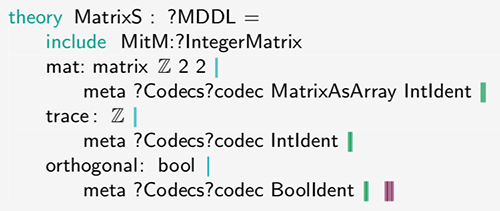
\includegraphics[width=.48\textwidth]{data_joe-schema}
  \caption{Schema theory for Joe's dataset}\label{fig:joe-schema}
\end{figure}

To fortify our intuition let us assume that Joe has collected a set of integer matrices together with their trace
and the Boolean property whether they are orthogonal.
Figure~\ref{fig:joe-schema} shows a MDDL theory that describes his database schema.
For example, the mathematical type of the field $\mathsf{mat}$ is integer $2\times2$ matrices;
the $\mathsf{codec}$ annotation specifies how this mathematical type is be encoded as a low-level database type (in this case: arrays of integers).
Concretely, the codec is $\mathsf{MatrixAsArray}$ codec operator applied to the identity codec for integers.
These codec annotations capture the representation theorem that allows representing the mathematical objects as ground data that can be stored in databases. 
%The tag \textsf{opaque} specifies that matrices cannot be used for filtering in the user interface. 

The information is sufficient to generate a database schema -- here one table with columns $\mathsf{mat}$, $\mathsf{trace}$, and $\mathsf{orthogonal}$ -- as well as a database browser-like website frontend (see Figure~\ref{fig:joe}).
The generation of APIs for computational software such as computer algebra systems is also possible and currently under development. 

\begin{figure}[ht]
  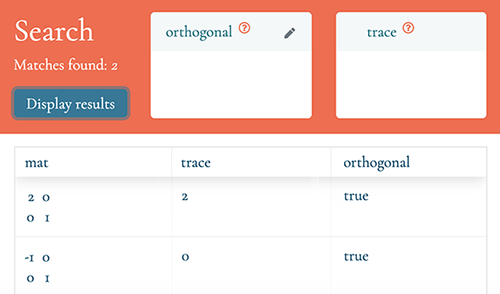
\includegraphics{data_joe.png}
  \caption{Website for Joe's dataset}\label{fig:joe}
\end{figure}

Crucially,  the codec-based setup transparently connects the mathematical level of specification with the database level -- a critical prerequisite for the deep FAIR properties postulated above.
Moreover, in Figure~\ref{fig:joe-schema}, the mathematical background knowledge is imported from a theory $\mathsf{IntegerMatrix}$ in the Math In The Middle ontology (MitM)~\cite{MitM:on}, which supplies the full mathematical specification and thus the basis for \emph{Interoperability} and \emph{Reusability}; see~\cite{BerKohRab:tumdi19,WieKohRab:vtuimkb17,KohMuePfe:kbimss17} for details.
The overhead of having to specify the semantics of the mathematical data is offset by the fact that we can reuse central resources like the MitM ontology and codec collection. 
Thus, MitM and MDDL form the nucleus of a common vocabulary for typical mathematical relational datasets. 
%These can and should eventually be linked to representation standards in other domains. 
%For mathematical datasets, the math-specific aspects attacked by our work are the dominant factor.

\paragraph{Web-Interface Analysis}
At the Workshop on Mathematical Data,
Andrea Kohlhase tested the user experience of the existing web interface
through user interviews.
The list of issues identified through the interviews is available at the 
workshop repository\footnote{https://github.com/OpenDreamKit/MathDataWorkshop/issues/3}.
Andrea Kohlhase also produced a clickable prototype of an updated interface
and used that in a few interviews combined with an eye-tracker test.




%%% Local Variables:
%%% mode: latex
%%% mode: visual-line
%%% fill-column: 5000
%%% TeX-master: "report"
%%% End:

%  LocalWords:  flexiformal BerKohRab:tumdi19 includegraphics textwidth textbf textsf textsf textsf ednote BerKohRab:tumdi19,WieKohRab:vtuimkb17,KohMuePfe:kbimss17 externalize
